\subsection{国际象棋环境}
\label{subsec:chess}
\begin{wrapfigure}{r}{0.5\columnwidth}
\vspace{-3ex}
    \centering
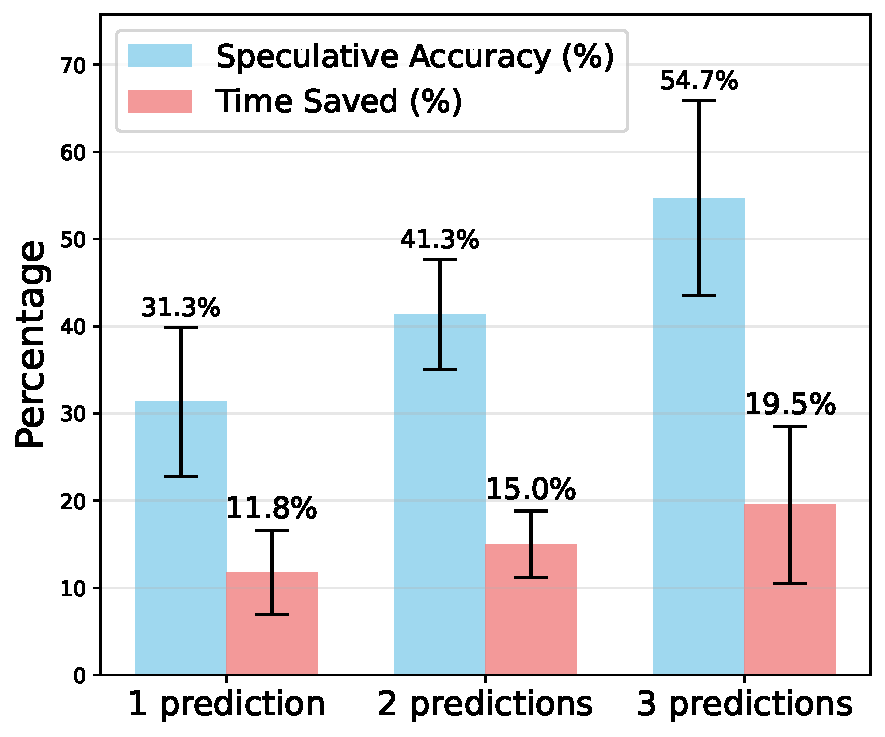
\includegraphics[width=0.9\linewidth]{figures/chess/combined_bar_plots.pdf}
  \caption{在 $30$ 个步数、共 $5$ 次运行上的节省时间比例与正确预测比例。}
  \vspace{-2em}
  \label{fig:chess_bar_plots}
\end{wrapfigure}

我们在竞争性多智能体博弈场景中展示该框架的有效性，并以国际象棋这一典型回合制任务作为例子。在标准对弈中，分析过程是严格串行的：每位玩家都只能在\textit{对手完成其回合之后}才开始思考。这样的串行化会引入大量空闲等待时间。尤其当双方都依赖计算量较大的推理模型时，一盘棋的实际耗时可能被拉长到数小时。我们的框架通过推测式并行分析放宽了这一限制，使玩家可以提前预判并准备对手最可能的走法。我们将表明，这能显著缩短整盘对局的总时长。

\subsubsection{实现}

我们基于 TextArena \citep{guertler2025textarena} 实现该框架；它为 LLM 驱动的智能体提供了标准化的博弈接口。

\textbf{推测流水线。} 在回合 $t$，游戏状态 $s_t$ 对应当前棋盘局面。当前行棋玩家发起一次 API 调用 $h_t$，其参数 $q_t$ 由 $s_t$ 与一条引导推理的提示词共同构成。此时玩家 $P$ 负责落子，玩家 $Q$ 等待。我们的框架按如下方式运行：
\begin{itemize}[leftmargin=*]
    \item \textbf{当前行棋玩家 $P$：} 玩家接收 $s_t$，并向智能体发起 API 调用 $h_t$，其中参数 $q_t = (s_t,\text{prompt})$。该调用返回下一步走法 $a_t = h_t(q_t)$。由于需要深度、充分的推理，这一步通常具有较高延迟。
    \item \textbf{未轮到行动的玩家 $Q$：}
    \begin{enumerate}
        \item \textbf{预测阶段。} Speculator 同样接收棋盘状态 $s_t$，并发起一次 API 调用 $\hat{h}_t$，但使用的是针对速度而非深度优化的提示词。它返回按置信度排序的 top-$k$ 走法预测 $\hat{a}_t^{(1)}, \hat{a}_t^{(2)}, \dots, \hat{a}_t^{(k)}$。
        \item \textbf{并行计算。} 对每个预测走法 $\hat{a}_t^{(i)}$，未行动玩家 $Q$ 会立刻启动一个并行进程，分析下一步应对走法 $\hat{a}_{t+1}^{(i)} = h_{t+1}(\hat{s}_{t+1}^{(i)},\text{prompt})$，其中 $i \in \{1,\ldots,k\}$，而 $\hat{s}_{t+1}^{(i)} = f(s_t,\hat{a}_t^{(i)})$ 表示将预测动作 $\hat{a}_t^{(i)}$ 作用于 $s_t$ 后得到的下一状态。
        \item \textbf{验证。} 当当前行棋玩家 $P$ 完成推理并返回其走法 $a_t$ 后，我们立即检查该走法是否与某个预测走法 $\hat{a}_t^{(1)}, \hat{a}_t^{(2)}, \dots, \hat{a}_t^{(k)}$ 相匹配。
        \item \textbf{提交或重启。} 若存在匹配，我们就提交相应的推测分支，直接推进到 $s_{t+1} = f(s_t, a_t)$，并终止其他线程。若没有匹配，则丢弃所有推测分支，并继续正常计算玩家 $Q$ 的正式走法 $a_{t+1} = h_{t+1}(f(s_t,a_t),\text{prompt})$。
    \end{enumerate}
\end{itemize}

这一流水线是\textit{无损的}：最终轨迹与不使用推测的对弈完全一致，但由于推理被并行化，整体耗时更短。

\textbf{智能体配置。} 我们发现，对 Speculator 与 Actor 使用同一个模型、但搭配不同提示词，可以在保持推测快速的同时最大化预测准确率。因此，在实验中，Actor 采用高推理强度的 GPT-5，每一步走法都通过一次 API 调用产生；Speculator 同样使用 GPT-5，但配置为低推理强度，并配合一条专为快速走法预测而非穷尽分析设计的系统提示词。

\subsubsection{结果}
我们从节省时间与预测准确率两个角度评估该框架。

我们跟踪两个指标：(i) 预测准确率，即在多少比例的回合中，至少有一个推测结果与真实走法一致；(ii) 节省时间，定义为 $(T_{\mathrm{seq}}-T_{\mathrm{s}})/T_{\mathrm{seq}}$，其中 $T_{\mathrm{s}}$ 和 $T_{\mathrm{seq}}$ 分别表示推测执行与顺序执行所需时间。

\textbf{预测越多，节省时间和准确率越高。}
\cref{fig:chess_bar_plots} 展示了 30 步对弈下的结果。与顺序对弈相比，我们的框架始终能够缩短执行时间，而且随着推测候选数增加，收益也随之增加。在 5 次运行中，使用 3 个预测时，平均节省时间为 $19.5\%$，平均预测准确率为 $54.7\%$。

\textbf{博弈中智能体调用的随机性。}
\cref{fig:chess_bar_plots} 中的方差反映了真实 API 调用下的实际对局动态。即便预测正确，节省的时间也不固定：如果落子后的局面存在显而易见的应对，那么无论是否推测，后续计算本来就会很快，因此加速效果有限。只有当预测通向需要深度分析的局面时，才会带来显著收益。因此，推测的效果同时取决于预测准确率以及所产生局面的复杂度。
